\documentclass{article}

\usepackage{graphicx}
\usepackage{tikz}
\usepackage{tikzsymbols}
\usetikzlibrary{calc,patterns,shapes.geometric}
\pagestyle{empty}
\usepackage[margin=0pt]{geometry}
\geometry{papersize={14in,12in}}

\def\centerarc[#1](#2)(#3:#4:#5){\draw[#1] ($(#2)+({#5*cos(#3)},{#5*sin(#3)})$) arc (#3:#4:#5);}

\begin{document}
	\begin{figure}
		\centering
		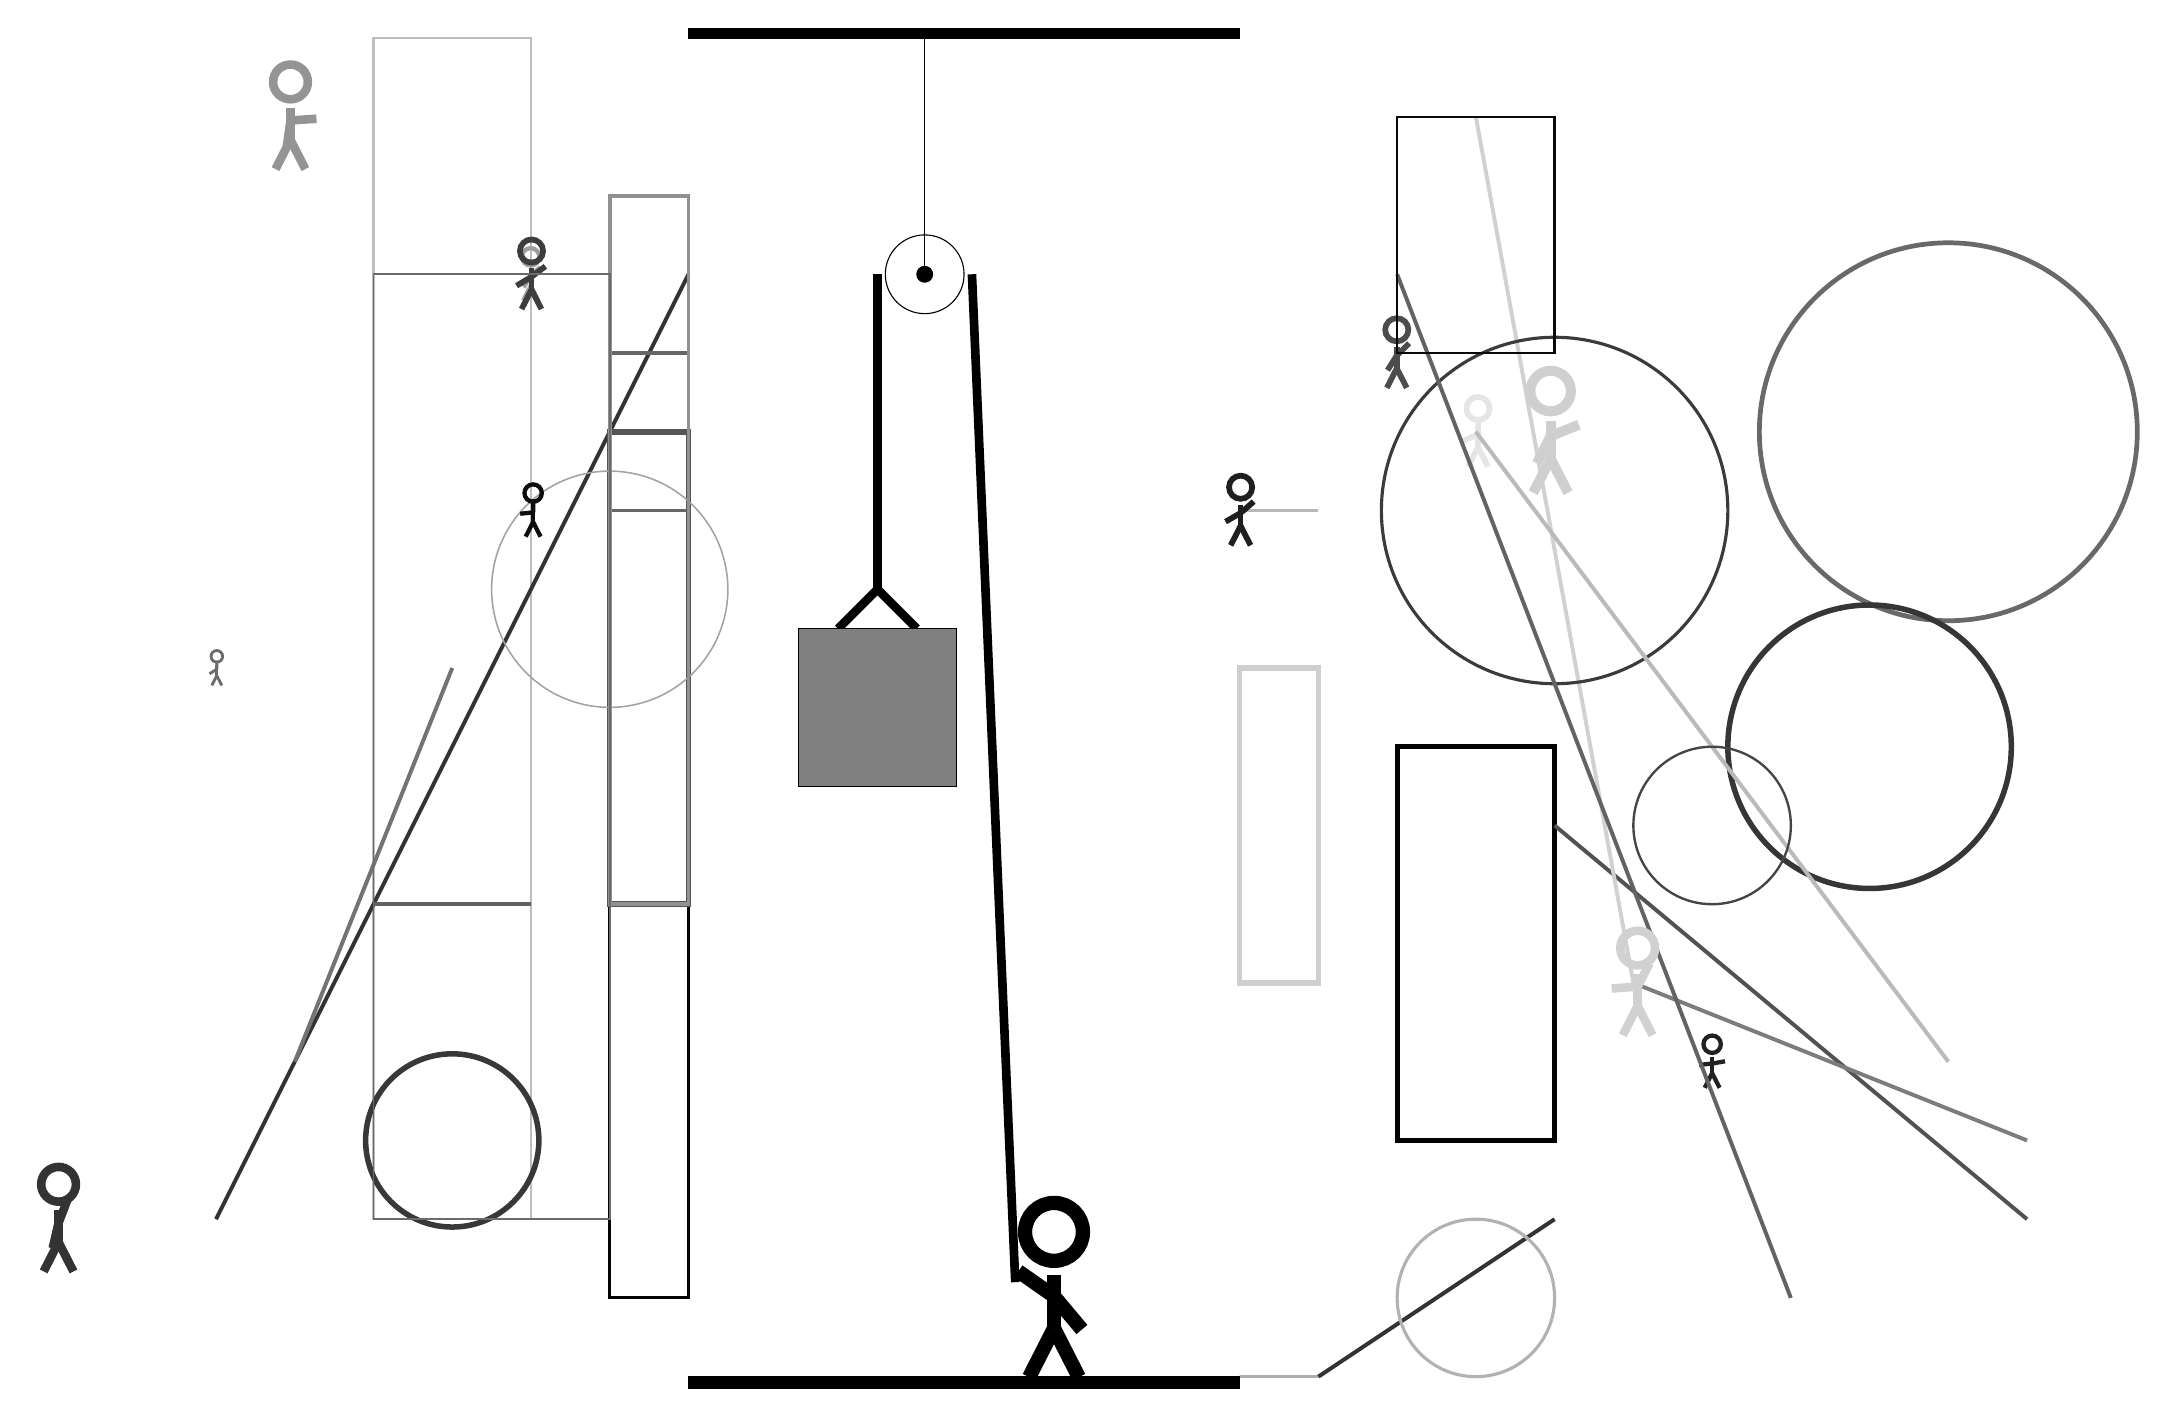
\begin{tikzpicture}
			%%%%% START %%%%%
			
			\draw[fill=black] (-2, 14) rectangle (5, 14.125);
			
			\draw (1, 11) circle (0.5);
			\draw[fill=black] (1, 11) circle (0.1);
			\draw (1, 14) -- (1, 11);
			
			\draw[line width=1.1mm] (-0.1, 6.5) -- (0.4, 7.0) -- (0.9, 6.5);
			\draw[fill=black!50] (-0.6, 6.5) rectangle (1.4, 4.5);
			
			\draw[line width=1.1mm] (0.4, 11) -- (0.4, 7.0);
			\centerarc[line width=1.1mm](1, 11)(0:180:0.6);
			\draw[line width=1.1mm](1.6, 11) -- (2.15, -1.8);
			
			\draw[line width=0.3mm, color=black!26] (-4, 14) rectangle (-6, -1);
			
			\node[line width=0.5mm, color=black!42] at (-7, 13) {\Strichmaxerl[6][82][4]};
			\draw[line width=0.5mm, color=black!28](6, 8) -- (5, 8);
			\draw[line width=0.4mm, color=black!98] (-3, 10) rectangle (-2, -2);
			\draw[line width=0.5mm, color=black!80](-2, 11) -- (-8, -1);
			\draw[line width=0.6mm, color=black!99] (7, 0) rectangle (9, 5);
			\draw[line width=0.5mm, color=black!68](9, 4) -- (15, -1);
			\draw [line width=0.6mm, color=black!44](10, -3) circle (0.0);
			\node[line width=0.7mm, color=black!70] at (7, 10) {\Strichmaxerl[4][58][45]};
			\node[line width=0.5mm, color=black!87] at (11, 1) {\Strichmaxerl[3][6][10]};
			\draw[line width=0.5mm, color=black!51](10, 2) -- (15, 0);
			
			\draw[line width=0.5mm, color=black!18](8, 13) -- (10, 2);
			\draw[line width=0.7mm, color=black!19] (6, 2) rectangle (5, 6);
			\draw[line width=0.7mm, color=black!67] (-3, 3) rectangle (-2, 9);
			\draw[line width=0.5mm, color=black!60] (-2, 8) rectangle (-3, 10);
			\draw[line width=0.4mm, color=black!32] (5, -3) rectangle (6, -3);
			\node[line width=0.4mm, color=black!58] at (-8, 6) {\Strichmaxerl[2][32][89]};
			\draw [line width=0.2mm, color=black!36](-3, 7) circle (1.5);
			\node[line width=0.7mm, color=black!38] at (-4, 11) {\Strichmaxerl[3][58][44]};
			
			\node[line width=0.7mm, color=black!19] at (9, 9) {\Strichmaxerl[7][63][22]};
			\draw[line width=0.5mm, color=black!62](-6, 3) -- (-4, 3);
			
			\draw [line width=0.6mm, color=black!59](14, 9) circle (2.4);
			\node[line width=0.7mm, color=black!80] at (-10, -1) {\Strichmaxerl[6][77][69]};
			\draw [line width=0.4mm, color=black!77](9, 8) circle (2.2);
			\draw[line width=0.5mm, color=black!55](-5, 6) -- (-7, 1);
			
			\draw [line width=0.7mm, color=black!79](13, 5) circle (1.8);
			\node[line width=0.7mm, color=black!10] at (8, 9) {\Strichmaxerl[4][24][89]};
			\draw[line width=0.5mm, color=black!61](7, 11) -- (12, -2);
			
			\draw [line width=0.7mm, color=black!78](-5, 0) circle (1.1);
			\node[line width=0.6mm, color=black!76] at (-4, 11) {\Strichmaxerl[4][31][37]};
			\draw[line width=0.5mm, color=black!43] (-3, 3) rectangle (-2, 12);
			
			\draw[line width=0.2mm, color=black!58] (-3, 11) rectangle (-6, -1);
			\draw[line width=0.5mm, color=black!27](8, 9) -- (14, 1);
			
			\node[line width=0.6mm, color=black!95] at (-4, 8) {\Strichmaxerl[3][6][89]};
			
			\node[line width=0.5mm, color=black!88] at (5, 8) {\Strichmaxerl[4][30][41]};
			\draw[line width=0.5mm, color=black!80](6, -3) -- (9, -1);
			
			\node[line width=0.5mm, color=black!18] at (10, 2) {\Strichmaxerl[6][4][63]};
			\draw[line width=0.3mm, color=black!96] (7, 10) rectangle (9, 13);
			\draw [line width=0.4mm, color=black!30](8, -2) circle (1.0);
			\draw [line width=0.3mm, color=black!73](11, 4) circle (1.0);
			
			\node at (2.6, -1.9) {\Strichmaxerl[10][-35][-50]};
			
			\draw[fill=black] (-2, -3) rectangle (5, -3.15);
			
			%%%%% END %%%%%
		\end{tikzpicture}
	\end{figure}	
\end{document}